\documentclass[12pt]{article}
\usepackage{amsmath,amsfonts,amsthm,fullpage,amssymb}
\usepackage{algorithm}
\usepackage{algorithmic}
\usepackage{graphicx}
\usepackage{url}

\usepackage{mdframed}
\usepackage{dsfont}
\usepackage{enumitem}
\usepackage{pdfpages}


\begin{document}

\title{ISYE 6740, Summer 2025, Homework 4\\{\small 100 points}}
\author{Prof. Yao Xie}
\date{}
\maketitle

\textbf{Provided Data:}
\begin{itemize}
    \item Q1: Comparing multi-class classifiers for MNIST Datasets [mnist\_10digits.mat, fashion-mnist\_train.csv, fashion-mnist\_test.csv]
\end{itemize}

\subsection*{1. Comparing multi-class classifiers for MNIST Datasets. (20 points)}

This question will compare different classifiers and their performance for multi-class classifications on the complete MNIST dataset, looking at both MNIST\_Digits and MNIST\_Fashion. Use the data files provided in the homework folder. Both MNIST datasets have 60,000 training examples and 10,000 test examples. We will compare {\bf KNN, logistic regression, SVM, kernel SVM, and neural networks}. 

\begin{itemize}[noitemsep]

\item Use 6740 as your random\_state / random seed
\item You should standardize the data before training your classifiers by mapping the range from [0,255] to [0,1].

\item You will run your models on both MNIST\_DIGITS and MNIST\_FASHION. The shape of your data after loading should be as follows:
    \begin{itemize}
        \item xtrain (60000, 784)
        \item xtest (10000, 784)
        \item ytrain (60000,)
        \item ytest (10000,)
    \end{itemize}

\item load MNIST\_DIGITS using scipy.io.loadmat

\item Utilize the following models from sklearn: 
  \begin{itemize}
    \item LogisticRegression
    \item KNeighborsClassifier : Adjust K to obtain a reasonable result. Feel free to use any reasonable tuning methodology, only report your best K
    \item MLPClassifier : Use \textsf{hidden\_layer\_sizes = (20, 10)}
    \item SVC : Use this for both SVM and Kernel SVM. Randomly downsample the training data to size $m=5000$ for efficiency. For kernel SVM, use radial basis function kernel (rbf).
  \end{itemize}
\end{itemize}

Train the classifiers on the training dataset and evaluate them on the test dataset.

\begin{enumerate}

\item (10 points) Report the precision, recall, and F-1 score for each of the classifiers. The classification metrics should be reported for each class in the dataset. Provide these results for both the digits and fashion datasets.

 
\item (10 points) Discuss the performance of the classifiers. Include explanations both on comparing the 5 classifiers against each other for the individual datasets, and some insight into performance on the different datasets. Which model performed best on each dataset, and why might some models perform better than others?

 
\end{enumerate}


\subsection*{2. SVM (25 points).}

\begin{enumerate}
\item (5 points) Explain why can we set the margin $c = 1$ to derive the SVM formulation? Justify using a mathematical proof.

\item (5 points) Using Lagrangian dual formulation, show that the weight vector can be represented as
\[
w = \sum_{i=1}^n \alpha_i y_i x_i.
\]
where $\alpha_i \geq 0$ are the dual variables. What does this imply in terms of how to relate data to $w$?

\item (5 points) Explain why only the data points on the ``margin'' will contribute to the sum above, i.e., playing a role in defining $w$. Hint: use the Lagrangian multiplier derivation and KKT condition we discussed in class. 

\item Simple SVM by hand. 

Suppose we only have four training examples in two dimensions as shown in Fig. The positive samples at $x_1 = (0, 0)$, $x_2 = (2, 2)$ and negative samples at $x_3 = (h, 1)$ and $x_4 = (0, 3)$. 
%
\begin{center}
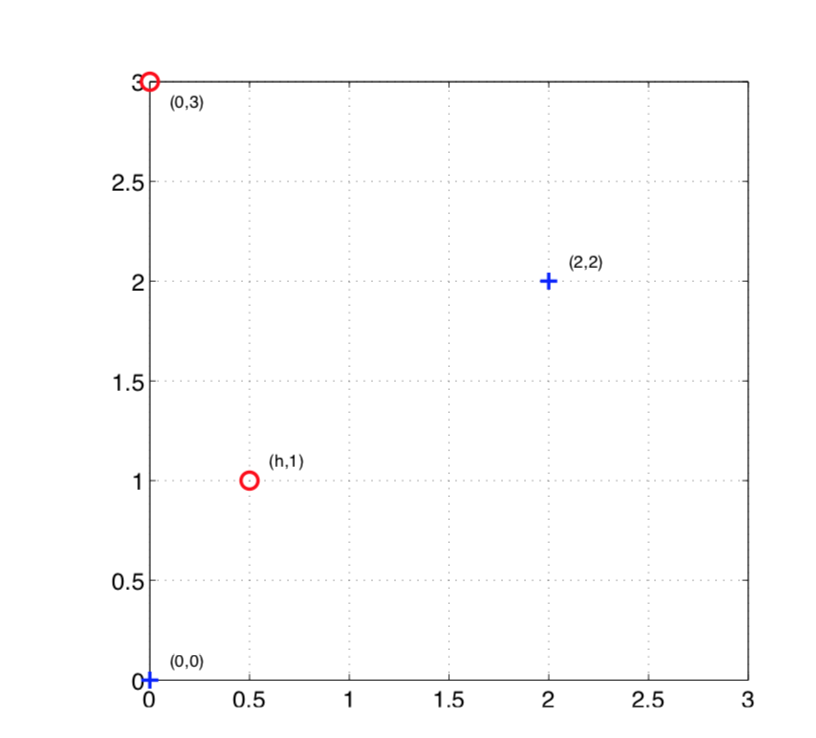
\includegraphics[width = 0.5\textwidth]{svm}
\end{center}

\begin{enumerate}
\item (5 points) For what range of parameter $h > 0$, the training points are still linearly separable? Be sure to consider all possible ranges.


\item (5 points) Does the orientation of the maximum margin decision boundary change as $h$ changes, when the points are separable? Please explain your conclusion.
\end{enumerate}


\end{enumerate}


\subsection*{3. Neural networks and backpropagation. (25 points)}


Consider a simple two-layer network in the lecture slides. Given $m$ training data $(x^i, y^i)$, $i = 1, \ldots, m$, the cost function used to training the neural networks
\[
\ell(w, \alpha, \beta) = \sum_{i=1}^m (y^i - \sigma(w^T z^i))^2
\]
where $\sigma (x) = 1/(1+e^{-x})$ is the sigmoid function, $z^i$ is a two-dimensional vector such that  $z_1^i = \sigma(\alpha^T x^i)$, and $z_2^i = \sigma(\beta^T x^i)$.
\\
Be sure to show all steps of your proofs.

\begin{enumerate}
\item (10 points) Show that the gradient is given by
\[
\frac{\partial \ell(w, \alpha, \beta) }{\partial w}
= - \sum_{i=1}^m 2(y^i - \sigma(u^i))\sigma(u^i)(1-\sigma(u^i)) z^i,
\]
where $u^i = w^T z^i$. 
\item (15 points) Also, show the gradient of $\ell(w, \alpha, \beta)$ with respect to $\alpha$ and $\beta$ and write down their expression.
\end{enumerate}

\subsection*{4. Feature selection and change-point detection. (30 points)} 

\begin{enumerate}

\item (15 points) Consider the mutual information-based feature selection. Suppose we have the following table (the entries in the table indicate counts) for the spam versus and non-spam emails:
%
\begin{center}
\begin{tabular}{c|c|c}
\hline
& ``prize'' = 1 & ``prize'' = 0 \\\hline
``spam'' = 1 & 130& 15 \\ \hline 
 ``spam'' = 0 & 1200 & 13000  \\\hline
\end{tabular}
\end{center}

\begin{center}
\begin{tabular}{c|c|c}
\hline
& ``hello'' = 1 & ``hello'' = 0 \\\hline
``spam'' = 1 & 160 & 25 \\ \hline 
 ``spam'' = 0 & 13000 & 7500  \\\hline
\end{tabular}
\end{center}

Given the two tables above, calculate the mutual information for the two keywords, ``prize`` and ``hello'' respectively. Which keyword is more informative for deciding whether or not the email is spam? If any tools are used for your calculation, you must still show your mathematical steps in your report and include code/files used for your calculations.

\item  (15 points)  Given two distributions, $f_0 = \mathcal{N}(0, 1)$, $f_1 = \mathcal{N}(0, 1.3)$, derive what should be the CUSUM statistic (i.e., show the mathematical CUSUM detection statistic specific to these distributions). Plot the CUSUM statistic for a sequence of 150 randomly generated i.i.d. (independent and identically distributed) samples, $x_1, \ldots, x_{100}$ according to $f_0$ and $x_{101}, \ldots, x_{150}$ according to $f_1$. Using your plot, please provide a reasonable estimation of where a change may be detected.\\
\textbf{Note: Be certain to set your random seed to 6740 to ensure reproducible results. Failure to do so will result in point deductions}


\end{enumerate}


\end{document}
